\section{CDS 15 Circular Postmark}

\begin{marginfigure}
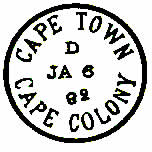
\includegraphics[width=.80\textwidth]{../cape-of-good-hope/circular-1869-1882/CDS-15.jpg}
\caption{CDS 15}
\end{marginfigure}



This postmark appears to be a little bit of a mystery. 
This is a circular datestamp used during late December 1881 to early January 1882 
and is use was limited to the Cape Town General Post Office. 

Goldblatt reports this as being used only for the back-stamping of letters. 
This was CDS 15 (Goldblatt p. 98). It is distinguished by its serified 
letters which were 3mm high. 
The diameter of the circle is 25 mm. Goldblatt noted two copies 
dated 1 and 6 January 1882. 

Putzel in his Postmarks of South Africa Vol. 2, Page 78 confirms the 
existence of four other examples. I have three examples as a backstamp dated Dec 81. 

The cover shown below (which appears to be unique) shows the Cape Town 
temporary Datestamp 
superbly struck as a despatch datestamp in greyish-black for JA 4 82 on 
3d pale claret (SG 39) 
cover to Kimberley, Diamond Fields. AT the back there is an arrival cds 
of JA 9 82. 

All these datestamps appear to have the time-control letter 'D' or 'L' 
used between 09.00-09.30 a.m.
 

     